\begin{frame}
    \frametitle{Experiments}
    \framesubtitle{Computational specs}


    UTFSM Cluster, GPU node. (Chile)
    \begin{table}[H]
        \centering
        \begin{tabular}{lr}
            \hline
            \emph{CPU} & Intel(R) Xeon(R) CPU X5650 @ 2.67GHz (24 cores) \\
            \emph{GPU} & Tesla M2050 @ 575 Mhz (448 cores). \\
            \emph{RAM} & 24 GB \\
            \emph{OS}  & Scientific Linux release 6.4 \\
            \hline
        \end{tabular}
        \caption{Hardware and Software settings.}
        \label{tab:hw}
    \end{table}

\end{frame}

\begin{frame}
    \frametitle{Experiments}
    \framesubtitle{Units and systems}

    \begin{itemize}
        \item Equal-mass Plummer sphere~\cite{plummer1911}.
        \item Standard {\nbody} units for the calculations and resulting output of
        the code~\cite{Henon,Heggie1986},

        \begin{block}{\red{{\nbody} Units}}
            \begin{itemize}
                \item Total mass, $\sum^{N}_{\rm i=0} m_{i} = 1$.
                \item Gravitational constant, $G=1$.
                \item Total energy, $E_{\rm tot} = K + U = -0.25$,
            \end{itemize}
        \end{block}
    \end{itemize}

\end{frame}

%\begin{frame}
%    \frametitle{Experiments}
%    \framesubtitle{}
%
%Besides the NBU, we also some time references in some test, just to check the some
%physical phenomena which occur in a given time. We define the \emph{half-mass
%relaxation time} as,
%
%\begin{align}
%    t_{\text{rh}} &= 0.138 \left( { N r_{h}^{3}\over Gm } \right)^{{1\over 2}}
%                      {1 \over \ln ( \gamma N ) },
%\end{align}
%
%\noindent
%where $r_{h}$ is the half-mass radius, and  $\Lambda = \gamma N$, argument of the
%Coulomb logarithm; to highlight physical phenomena, like the \emph{core collapse}.
%
%\end{frame}

\begin{frame}
    \frametitle{Experiments}
    \framesubtitle{$\eta$ and the energy conservation}

\begin{figure}[H]
    \centering
    \label{fig:eta_energy}
    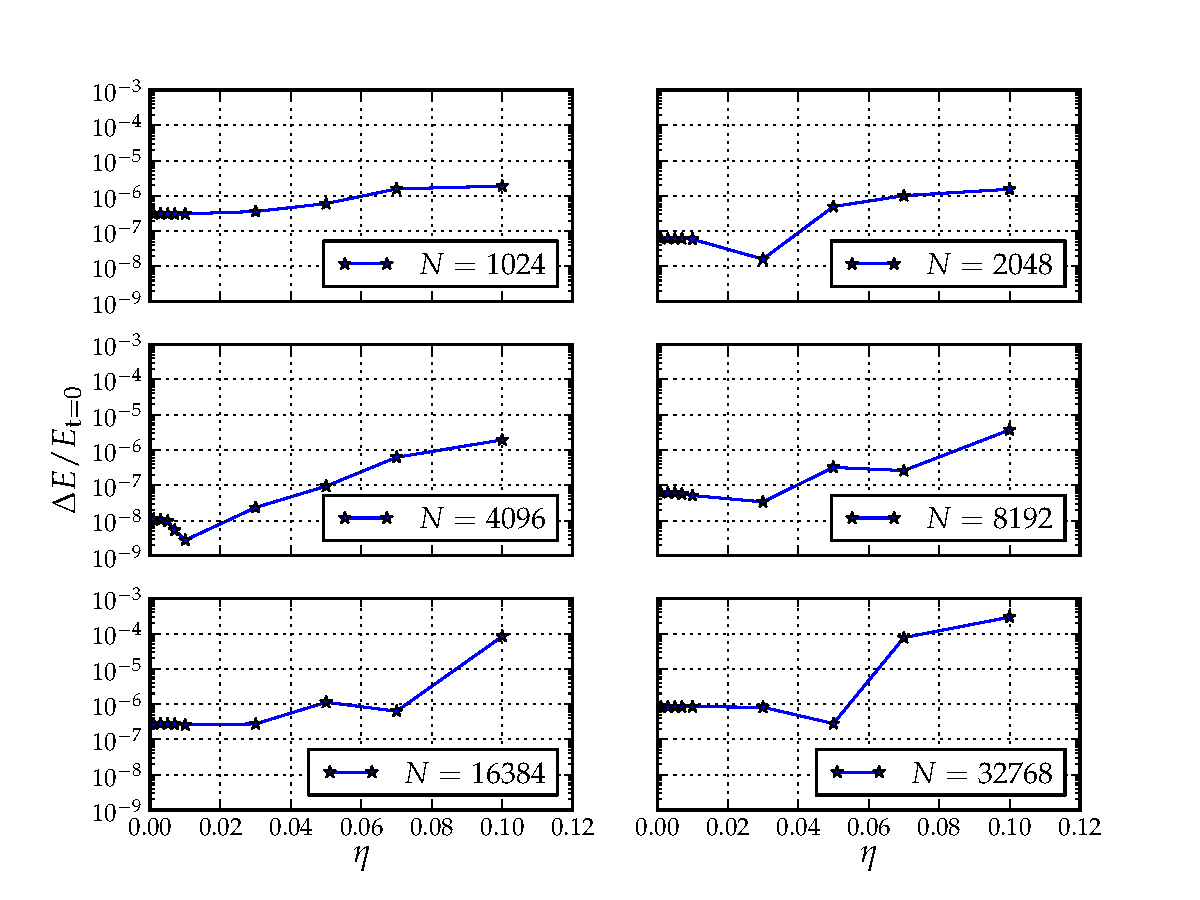
\includegraphics[width=0.65\textwidth]{img/test_energy_eta_N.pdf}
    \caption{Cumulative energy error up to $t=1$ NBU as a function of $\eta$.
             All the plots represent Plummer spheres with  different
             amount of particles.}
\end{figure}

\end{frame}

\begin{frame}
    \frametitle{Experiments}
    \framesubtitle{$\eta$ and the clock time}

\begin{figure}[H]
    \centering
    \label{fig:eta_time}
    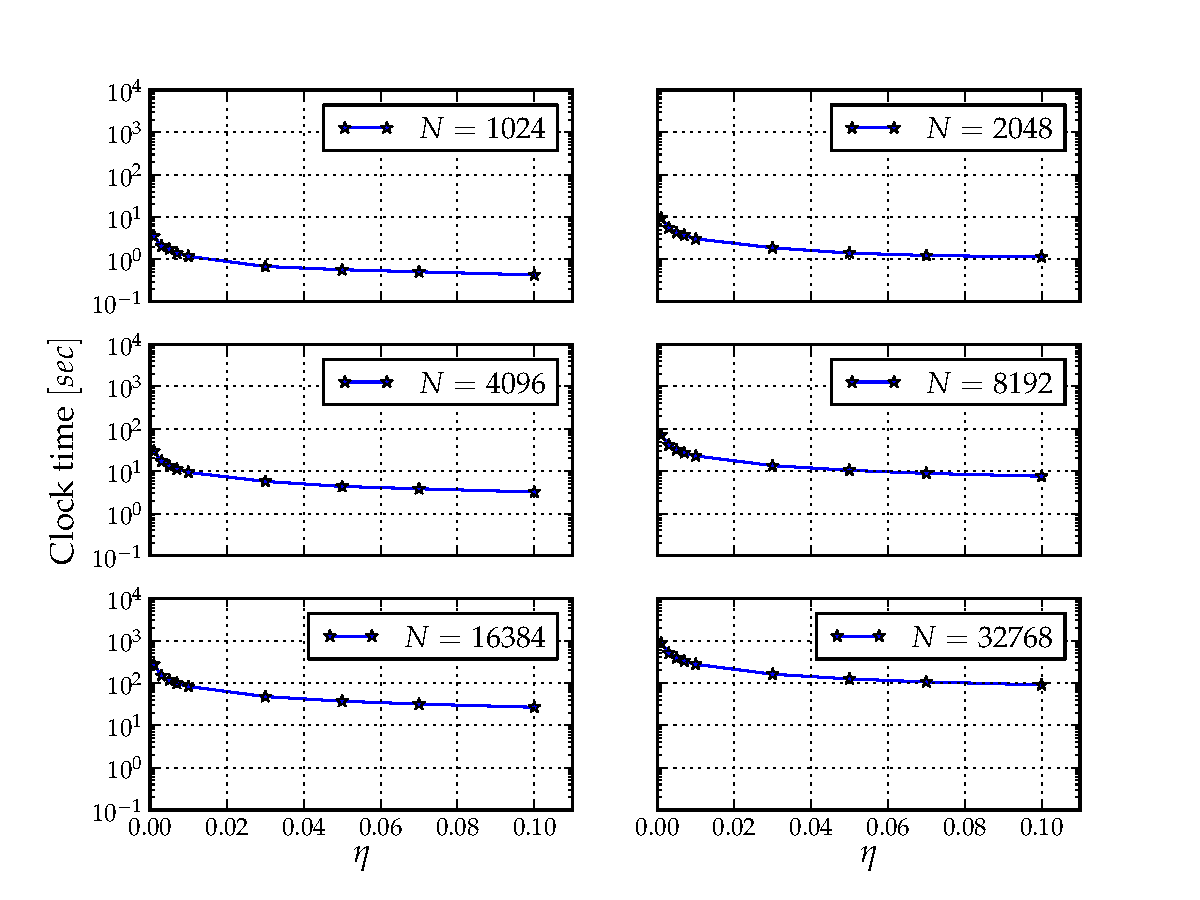
\includegraphics[width=0.65\textwidth]{img/test_time_eta_N.pdf}
    \caption{Clock time up to $t=1$ NBU as a function of $\eta$.
             All the plots represent Plummer spheres with  different
             amount of particles.}
\end{figure}

\end{frame}


\begin{frame}
    \frametitle{Experiments}
    \framesubtitle{Integrator scaling}

\begin{figure}[H]
    \centering
    \label{fig:time}
    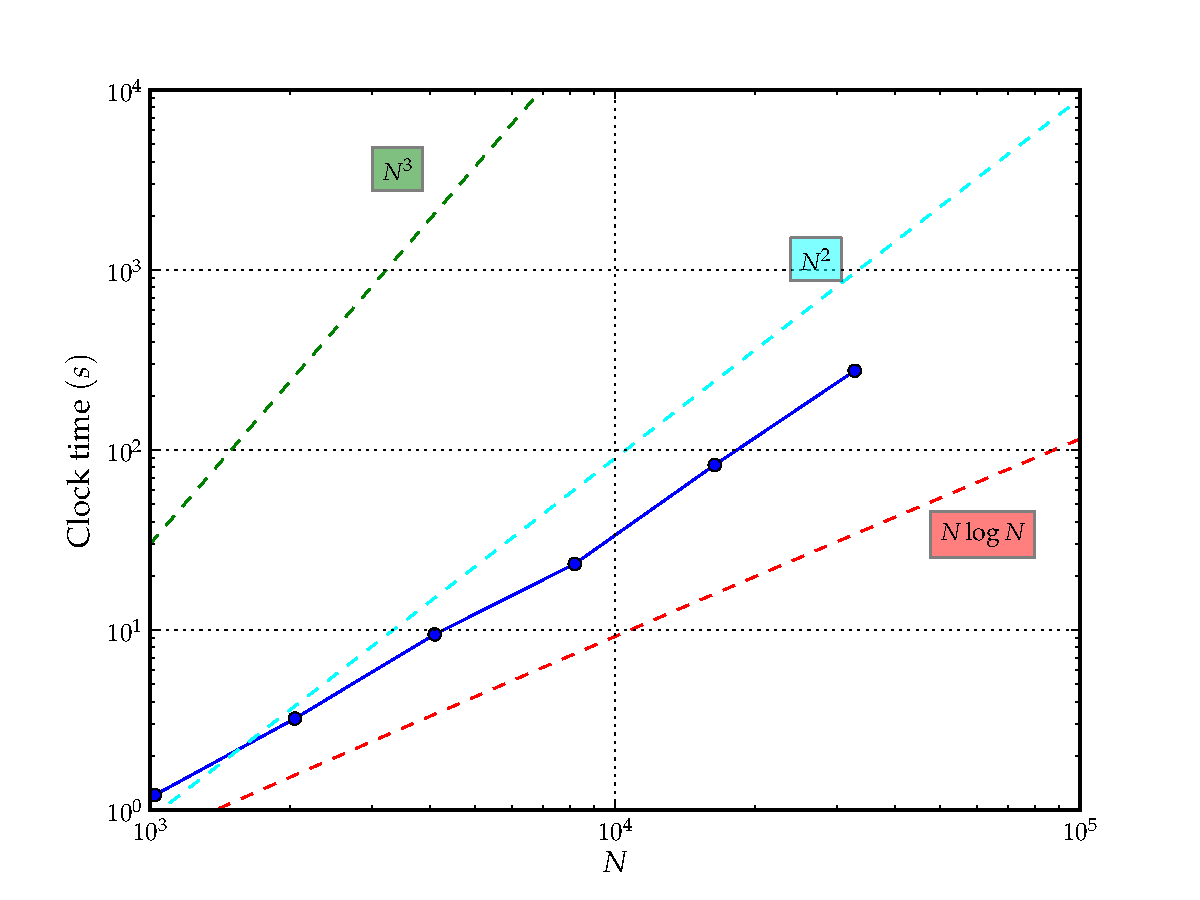
\includegraphics[width=0.65\textwidth]{img/test_time-1t-N.pdf}
    \caption{Clock time of integration up to $t=1$ NBU using $\eta = 0.01$ and
             $\epsilon = 10^{-4}$ using different amount of particles.}
\end{figure}

\end{frame}
\begin{frame}
    \frametitle{Experiments}
    \framesubtitle{Clock time comparison}


\begin{table}[H]
    \centering
    \footnotesize
    \begin{tabular}{rrrrr}
        \hline
        {\bf N} & \multicolumn{1}{c}{\bf CPU}
                & \multicolumn{1}{c}{\bf CPU + OpenMP}
                & \multicolumn{1}{c}{\bf CPU + GPU}
                & \multicolumn{1}{c}{\bf GPU}   \\
                & (single thread) & (many threads)     & (mixed approach) &  (multi threads) \\ \hline
         {\bf  1k} &    12.98 [s] &   8.19 [s] &    3.57 [s]           &    1.21 [s]          \\
         {\bf  2k} &    61.32 [s] &  34.94 [s] &   13.42 [s]           &    3.22 [s]          \\
         {\bf  4k} &   282.98 [s] & 162.64 [s] &   54.28 [s]           &    9.45 [s]          \\
         {\bf  8k} &  1227.40 [s] & 682.56 [s] &  208.91 [s]           &   23.31 [s]          \\
         {\bf 16k} &  5542.35 [s] & 3227.91 [s] &  904.82 [s]           &   82.63 [s]          \\
         {\bf 32k} & 26383.71 [s] & 15076.40 [s] & 3722.92 [s]           &  275.53 [s]          \\ \hline
    \end{tabular}
    \caption{Clock time foreach integrator version.}
    \label{tab:acc}
\end{table}

\end{frame}

\begin{frame}
    \frametitle{Experiments}
    \framesubtitle{Clock time comparison}

\begin{figure}[H]
    \centering
    \label{fig:acc}
    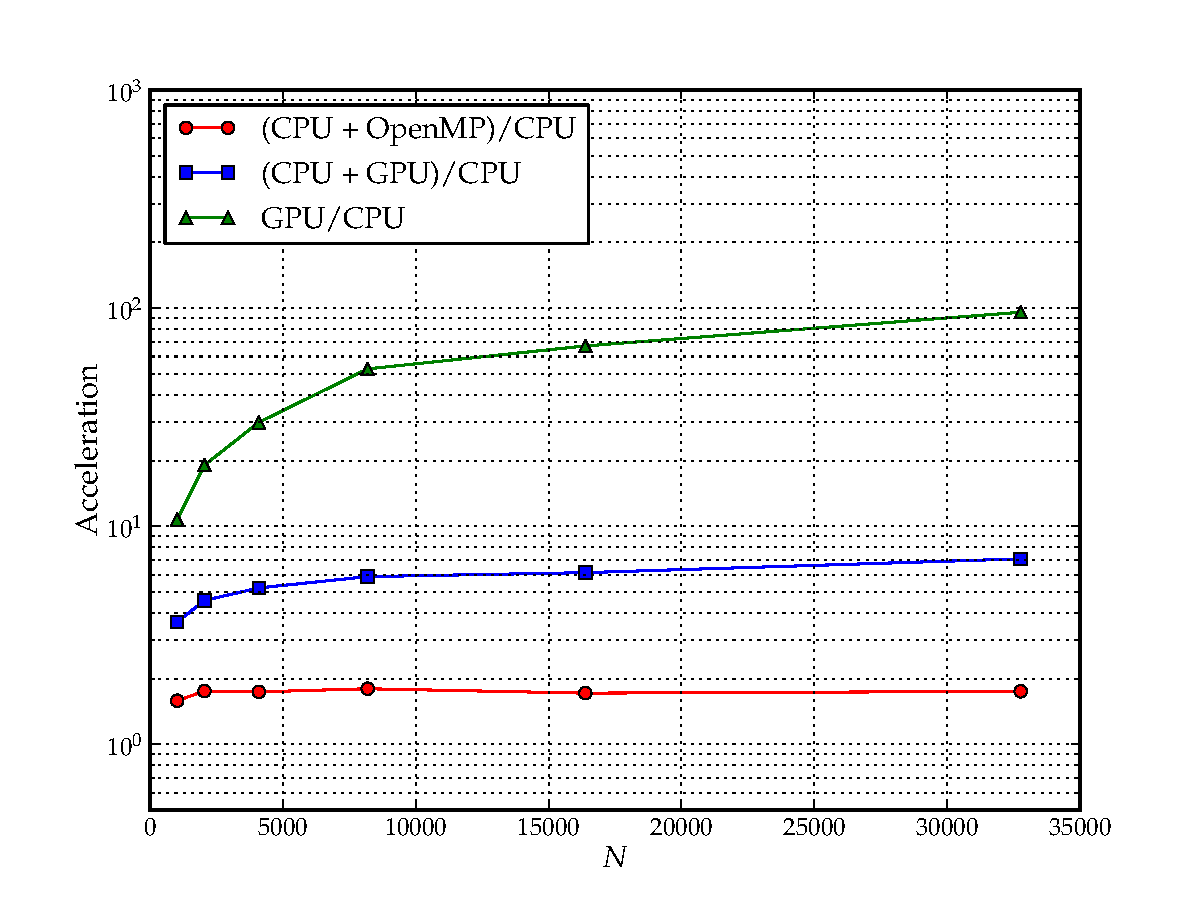
\includegraphics[width=0.7\textwidth]{img/test_gpu-acceleration.pdf}
    \caption{Acceleration between the implementations described in Table~\ref{tab:acc}}
\end{figure}

\end{frame}
\begin{frame}
    \frametitle{Experiments}
    \framesubtitle{Integrator Performance}
%The motivation of this thesis started of the work of Tsuyoshi Hamada,
%in his publications~\cite{Hamada42, Hamada190}, and later by Ishiyama
%et al.~\cite{Ishiyama4.45}, where with large GPU clusters was possible to achieve a
%huge amount of TFLOPS and PFLOPS, being even recognized with the ACM Gordon Bell
%Prize~\footnote{Website \url{http://awards.acm.org/bell/}}.

%We used the notation given by Berczik et al.~\cite{berczik2011high} (Eq. 17),

%\begin{equation}
%    P = \frac{(total flop operations)}{T_{\rm tot}} = \gamma\cdot N\cdot\sum N_{\rm act},
%\end{equation}

%\noindent
%where $\gamma$ is based on the gravitational interaction kernel flop count,
%that in this case is $\gamma = 60$; $N$ the total amount of particles in the system;
%$N_{\rm act}$ the particles to be updated in each iteration; and $T_{\rm tot}$
%the total elapsed time, in seconds.

\begin{figure}[H]
    \centering
    \label{fig:gflops}
    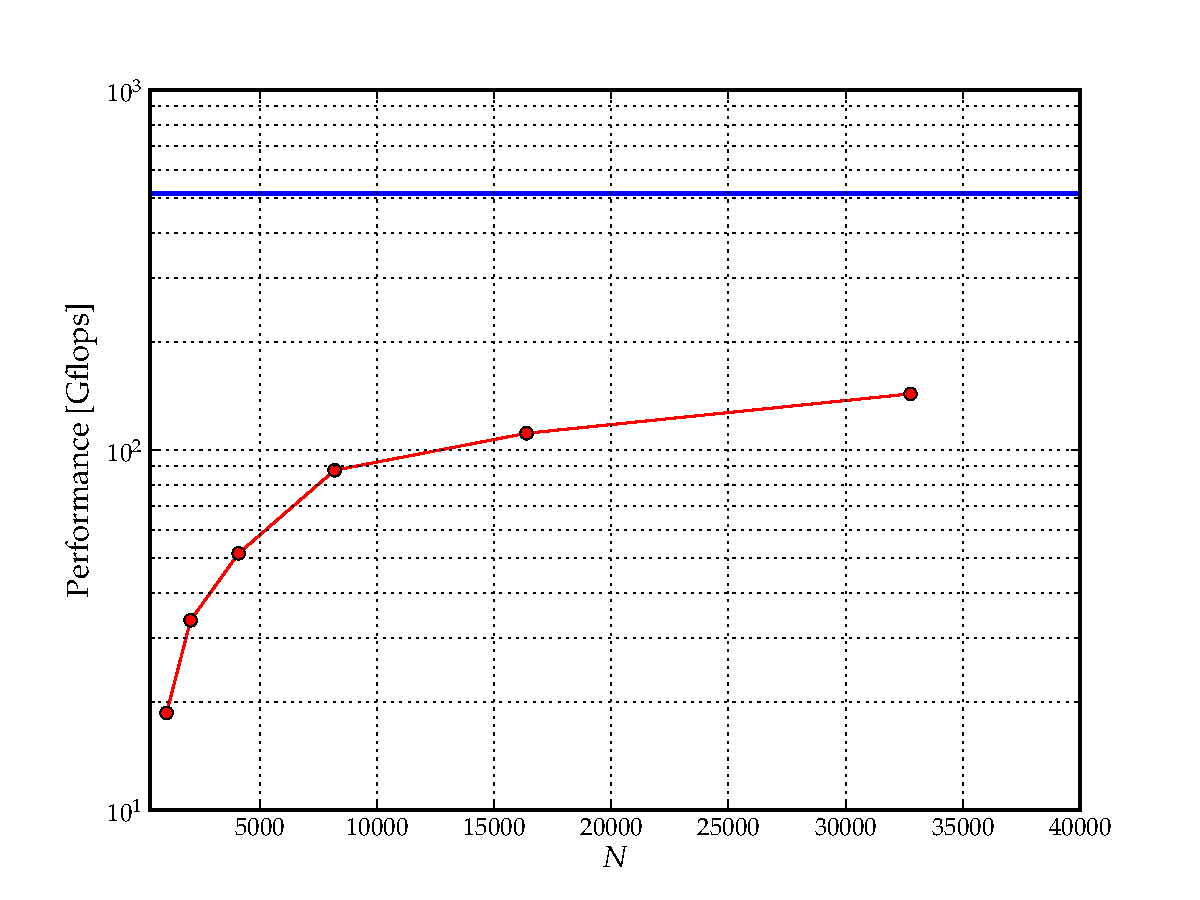
\includegraphics[width=0.65\textwidth]{img/test_gflops.pdf}
    \caption{GPU gravitational interactions performance in GFLOPS for different amount of particles.}
\end{figure}

\end{frame}
\begin{frame}
    \frametitle{Experiments}
    \framesubtitle{Lagrange radii}

%The \emph{Half-mass relaxation time} it is defined by:
%
%\begin{align}
%   t_{\rm rlx} =& 0.138 \left( \frac{Nr_{h}^{3}}{Gm} \right)^{1/2} \frac{1}{\ln(\gamma N},
%\end{align}
%
%\noindent
%where $\gamma N = \Lambda$ is the argument of the Coulomb logarithmic (historically
%$\gamma = 0.4$).

%And finally, a long-term time scale to determinate a physical phenomena
%called \emph{Core-collapse time} has been defined approximately as
%$t_{\rm cc} \approx 15 t_{\rm rlx}$.

\begin{figure}[h!t]
    \centering
    \label{fig:lagrangeradii}
    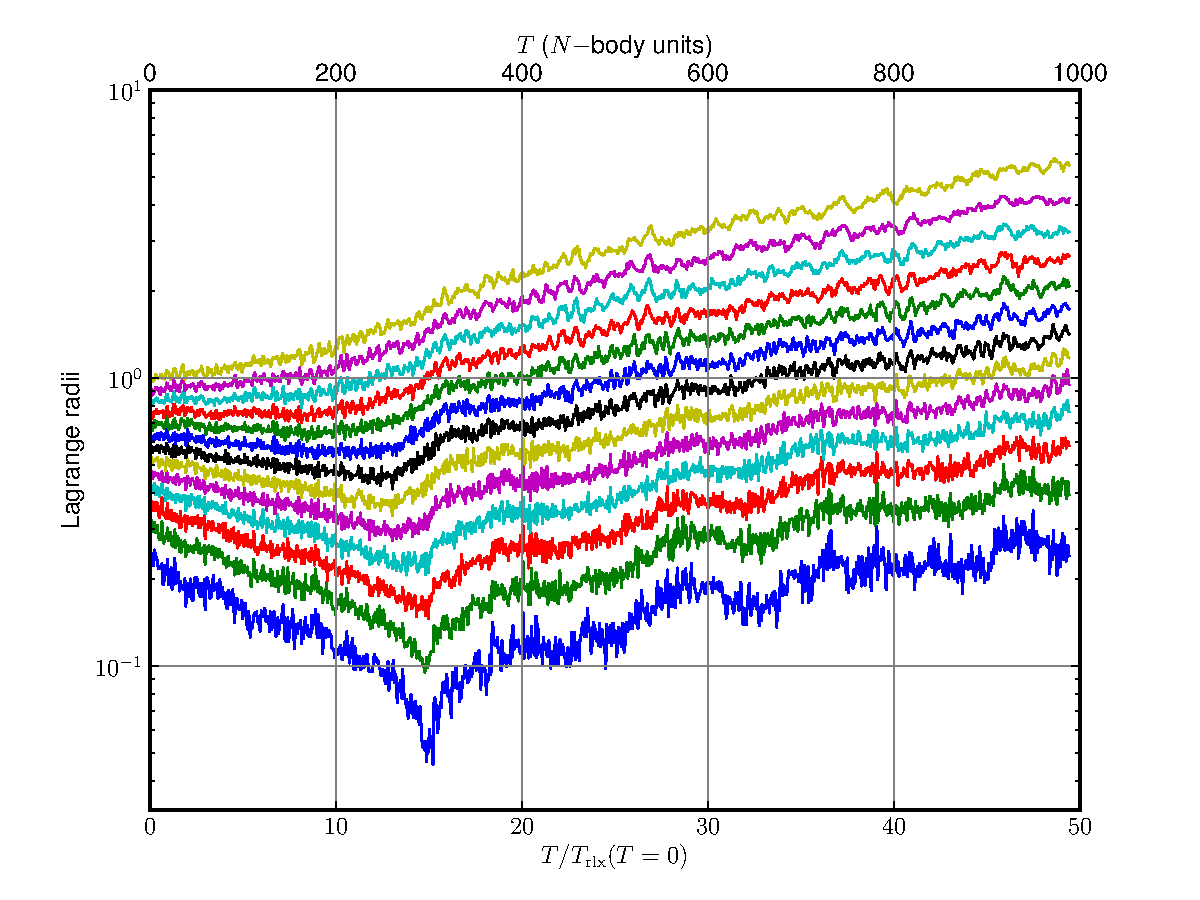
\includegraphics[width=0.55\textwidth]{img/lagrange_radii_1024_1000t.pdf}
    \caption{Lagrange radii of an {\nbody} system with 1024 particles.
             The radii distribution are  $5\%, 10\%, 15\%, \ldots, 65\%$ of the total mass.
             The core collapse is reached at $T_{\rm cc} \approx 15 T_{\rm rh}$.
             The half-mass relaxation time is $T_{\rm rh} = 20.24 [nbu]$}
\end{figure}


\end{frame}


\begin{frame}
    \frametitle{Experiments}
    \framesubtitle{Core radius and density evolution}

\begin{figure}[H]
    \centering
    \label{fig:core_p_r}
    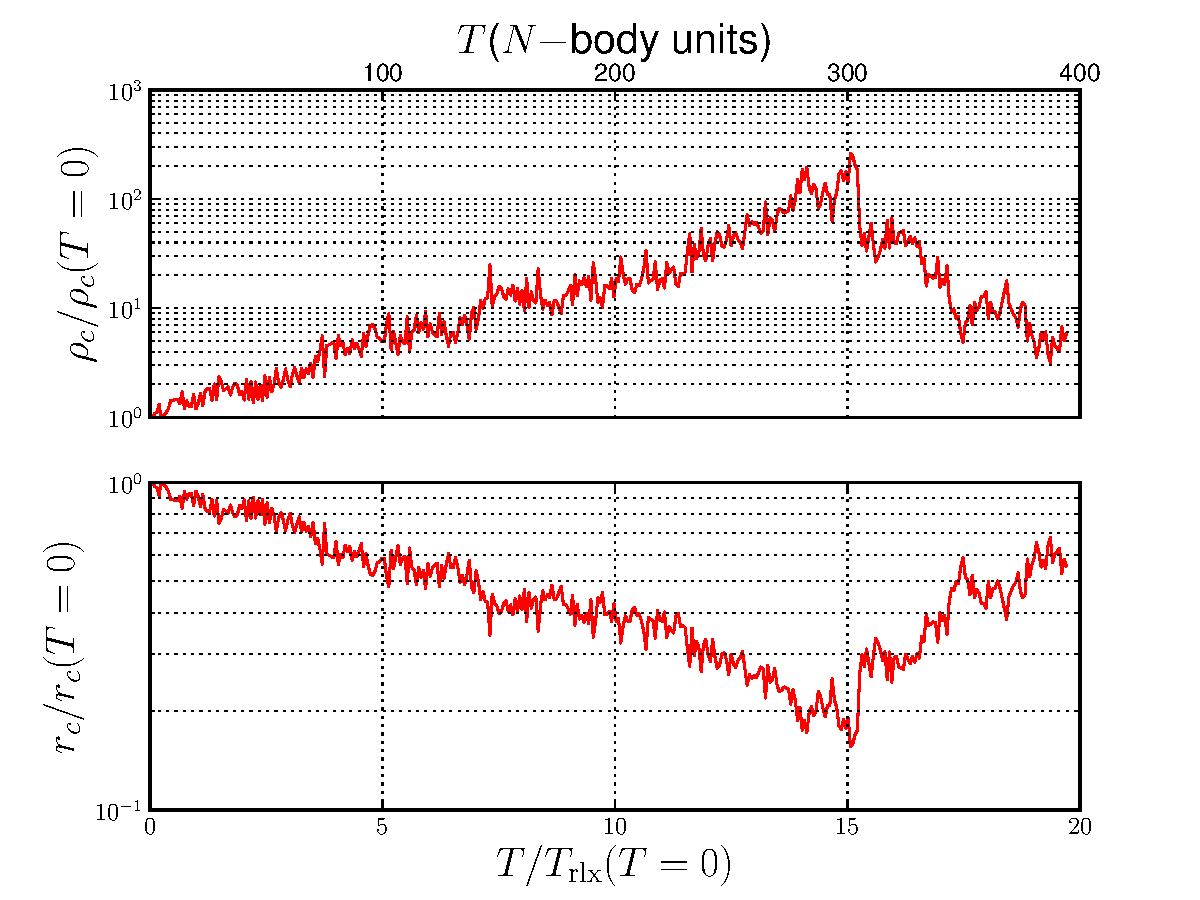
\includegraphics[width=0.65\textwidth]{img/test_density_core-radius_tcc_1k.pdf}
    \caption{Evolution of the core radius and core density until core collapse
             in a system with $N=1024$}
\end{figure}

\end{frame}
\begin{frame}
    \frametitle{Experiments}
    \framesubtitle{Long term integration}

\begin{figure}[h!t]
    \centering
    \label{fig:energy}
    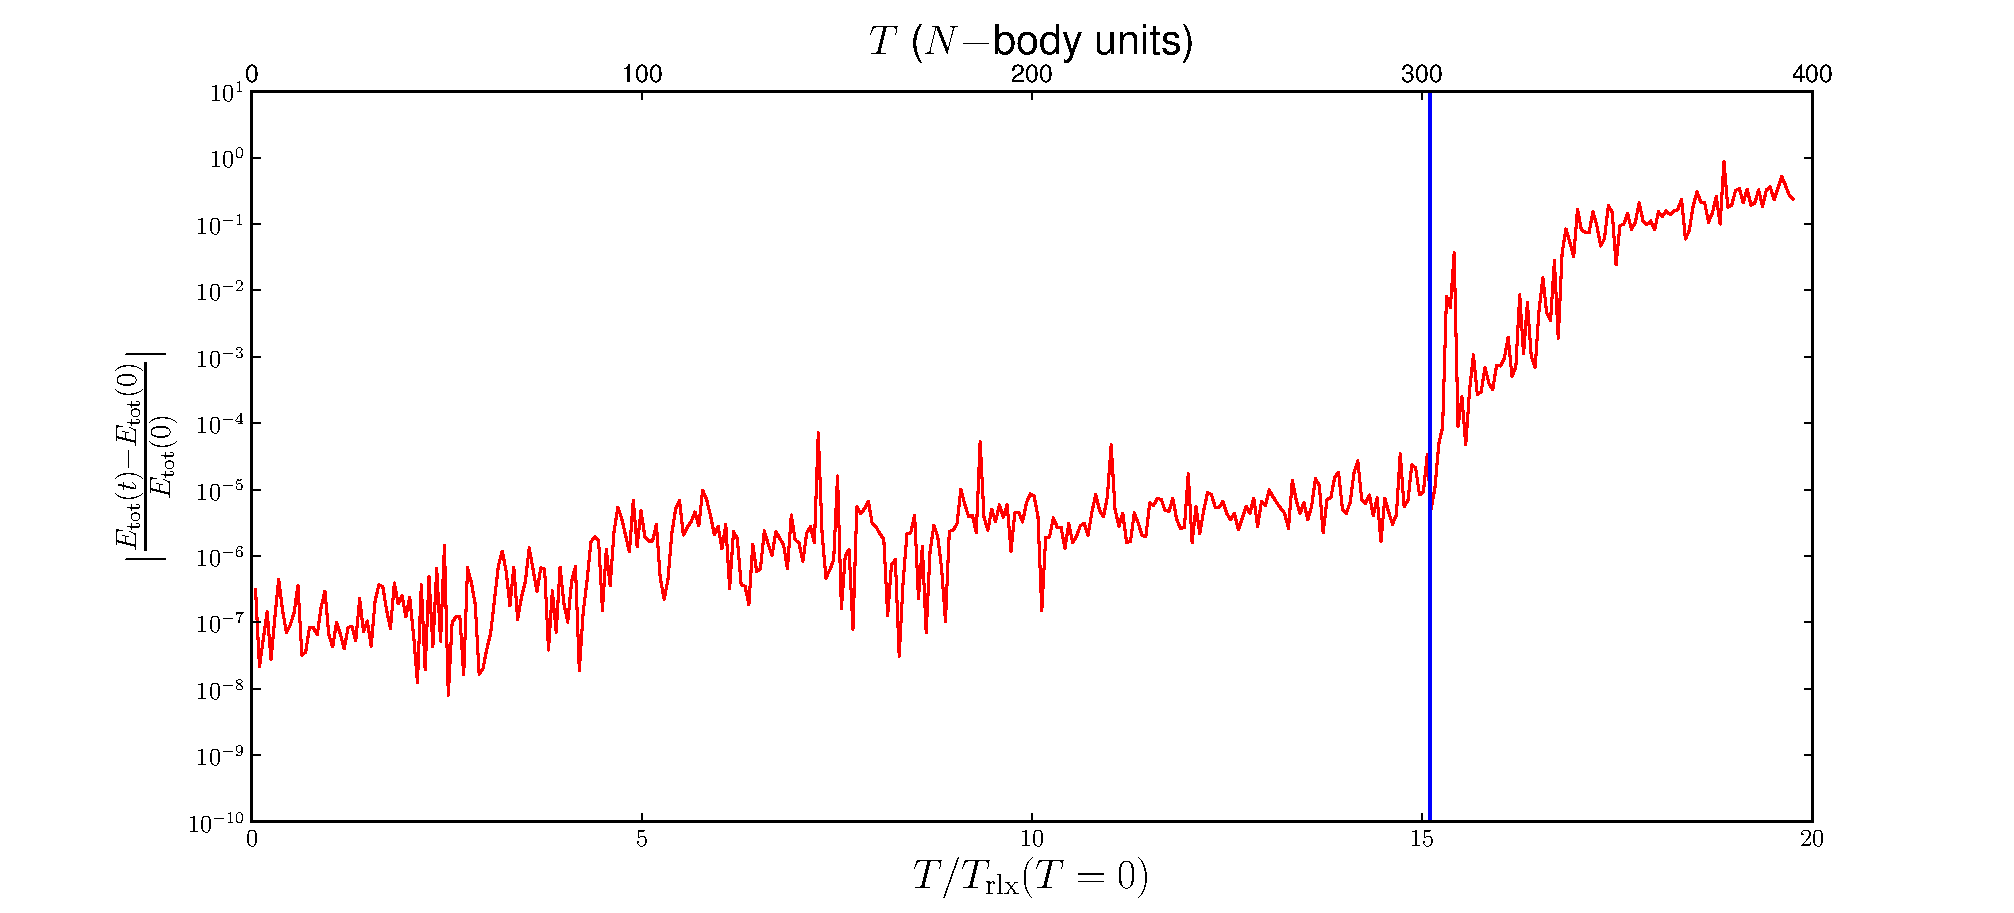
\includegraphics[width=0.9\textwidth]{img/test_energy-conservation_1k-400t.pdf}
    \caption{Energy conservation in a long time integration of a system with
             $N=1024$}
\end{figure}

\end{frame}
%\begin{frame}
%    \frametitle{Experiments}
%    \framesubtitle{}
%
%\begin{figure}{H}
%    \centering
%    \label{fig:dtdistribution}
%    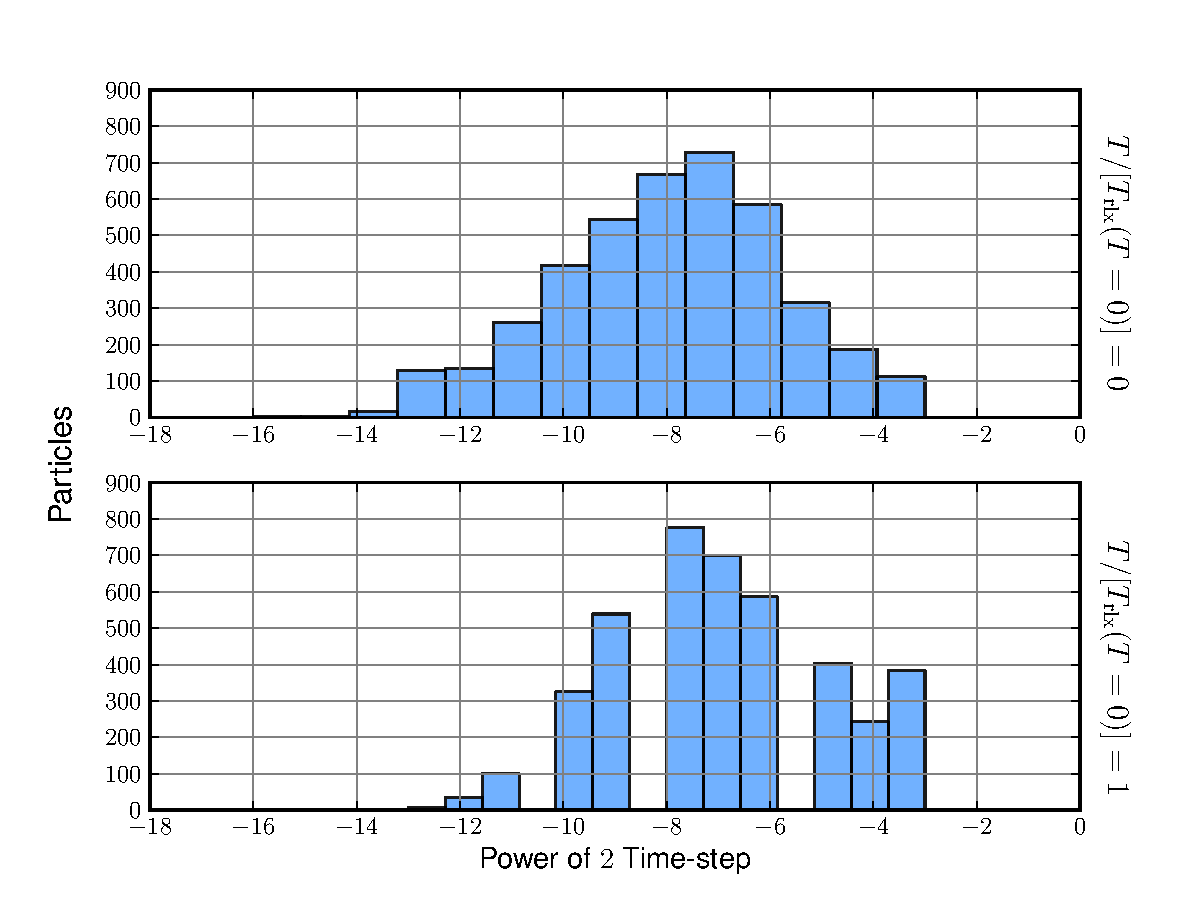
\includegraphics[width=0.8\textwidth]{img/test_dt_distribution.pdf}
%    \caption{Timestep distribution of a Plummer sphere with $4096$ particles,
%             before starting the integration $t=0$ and after 1 $T_{\rm rlx}$.}
%\end{figure}
%
%\end{frame}
